\documentclass[tikz,border=10pt]{standalone}
\usepackage{tikz}
\begin{document}
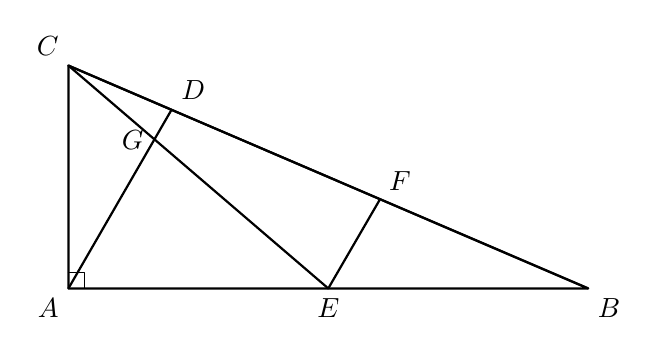
\begin{tikzpicture}[scale=1, line join=round, line cap=round]
  \coordinate (A) at (0,0);
  \coordinate (B) at (6.6,0);
  \coordinate (C) at (0,2.83);
  \coordinate (E) at (3.3,0);
  \coordinate (D) at (1.31,2.27);
  \coordinate (F) at (3.95,1.12);
  \coordinate (G) at (1.08,1.88);

  \draw[thick] (C) -- (A) -- (B) -- cycle;
  \draw[thick] (C) -- (B);
  \draw[thick] (A) -- (D);
  \draw[thick] (C) -- (E);
  \draw[thick] (E) -- (F);

  \draw (0.2,0) -- (0.2,0.2) -- (0,0.2);

  \node[above left] at (C) {$C$};
  \node[below left] at (A) {$A$};
  \node[below right] at (B) {$B$};
  \node[below] at (E) {$E$};
  \node[above right] at (D) {$D$};
  \node[above right] at (F) {$F$};
  \node[left] at (G) {$G$};
\end{tikzpicture}
\end{document}
